\section{Bodediagramm}

Beispiele verschiedener Bodediagramm und zugehötiger Pol-Nullstellen-Diagramme \\
siehe Skript, Kapitel 5.4.3 (S. 222)


\subsection{Approximationen im Bodediagramm}

\begin{minipage}[t]{0.48\columnwidth}
    \raggedright
    \subsubsection{Pol im Ursprung}

    \begin{outline}
        \1 $H(s) = \frac{\alpha}{s} \cbl{= \frac{2}{s}}$
            \2 Betrag $=$ Gerade mit Steigung $- 20 \, \deci \bel / \Dek$, Schnittpunkt mit $0 \, \deci\bel$-Linie bei $\omega = \alpha$
            \2 Phase $- \frac{\pi}{2} = \const$
    \end{outline}

    \begin{center}
    % Gain
    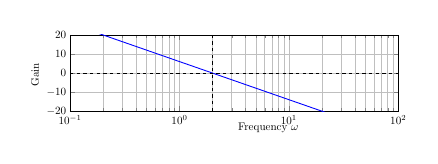
\begin{tikzpicture}
        [
            scale = 0.4,
            >=latex
        ]
        \begin{axis}
            [
                width=12cm,
                height=4cm,
                xmode=log,
                xmin=0.1, xmax=100, ymin=-20, ymax=20,
                x label style={anchor=west},
                xlabel=Frequency $\omega$,
                y label style={anchor=south},
                ylabel=Gain $\deci \bel$,
                xmajorgrids=true,
                xminorgrids=true,
                ymajorgrids=true
            ]

            \addplot[thick, color=blue, domain=0.1:100]{-20*log10(x)+6};

            \addplot[dashed, color=black, domain=0.1:100]{0};
            \addplot[dashed, color=black, domain=2:2] coordinates {(2, -20) (2, 20)};
        \end{axis}
        
    \end{tikzpicture}


    % Phase
    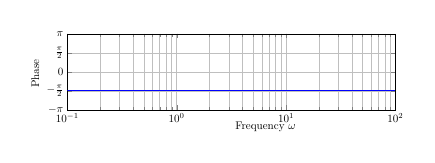
\begin{tikzpicture}
        [
            scale = 0.4,
            >=latex
        ]
        \begin{axis}
            [
                width=12cm,
                height=4cm,
                xmode=log,
                xmin=0.1, xmax=100, ymin=-3.141, ymax=3.141,
                x label style={anchor=west},
                xlabel=Frequency $\omega$,
                y label style={anchor=south},
                ylabel=Phase $\rad$,
                ytick={-3.14, -1.57, 0, 1.57, 3.14},
                yticklabels={$-\pi$, $-\frac{\pi}{2}$, $0$, $\frac{\pi}{2}$, $\pi$},
                xmajorgrids=true,
                xminorgrids=true,
                ymajorgrids=true
            ]
            
            \addplot[thick, color=blue, domain=0.1:100]{-1.57};     

        \end{axis}
            
    \end{tikzpicture}
\end{center}


\end{minipage}
\hfill
\begin{minipage}[t]{0.48\columnwidth}
    \raggedright
    \subsubsection{Nullstelle im Ursprung}

    \begin{outline}
        \1 $H(s) = \alpha \cdot s \cbl{= 3\cdot s}$
            \2 Betrag $=$ Gerade mit Steigung $+ 20 \, \deci \bel / \Dek$, Schnittpunkt mit $0 \, \deci\bel$-Linie bei $\omega = \frac{1}{\alpha}$
            \2 Phase $+ \frac{\pi}{2} = \const$
    \end{outline}

    \begin{center}
    % Gain
    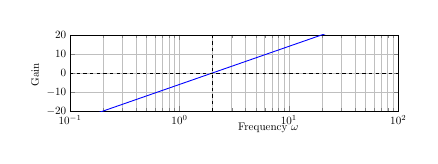
\begin{tikzpicture}
        [
            scale = 0.4,
            >=latex
        ]
        \begin{axis}
            [
                width=12cm,
                height=4cm,
                xmode=log,
                xmin=0.1, xmax=100, ymin=-20, ymax=20,
                x label style={anchor=west},
                xlabel=Frequency $\omega$,
                y label style={anchor=south},
                ylabel=Gain $\deci \bel$,
                xmajorgrids=true,
                xminorgrids=true,
                ymajorgrids=true
            ]

            \addplot[thick, color=blue, domain=0.1:100]{20*log10(x)-6};

            \addplot[dashed, color=black, domain=0.1:100]{0};
            \addplot[dashed, color=black, domain=2:2] coordinates {(2, -20) (2, 20)};
        \end{axis}
        
    \end{tikzpicture}


    % Phase
    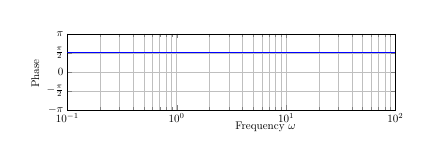
\begin{tikzpicture}
        [
            scale = 0.4,
            >=latex
        ]
        \begin{axis}
            [
                width=12cm,
                height=4cm,
                xmode=log,
                xmin=0.1, xmax=100, ymin=-3.141, ymax=3.141,
                x label style={anchor=west},
                xlabel=Frequency $\omega$,
                y label style={anchor=south},
                ylabel=Phase $\rad$,
                ytick={-3.14, -1.57, 0, 1.57, 3.14},
                yticklabels={$-\pi$, $-\frac{\pi}{2}$, $0$, $\frac{\pi}{2}$, $\pi$},
                xmajorgrids=true,
                xminorgrids=true,
                ymajorgrids=true
            ]
            
            \addplot[thick, color=blue, domain=0.1:100]{1.57};                 
        \end{axis}
            
    \end{tikzpicture}
\end{center}


\end{minipage}


\begin{minipage}[t]{0.48\columnwidth}
    \raggedright
    \subsubsection{Reeller Pol}

    \begin{outline}
        \1 $H(s) = \frac{\alpha}{s + \alpha} = \frac{1}{\frac{s}{\alpha} + 1} \cbl{= \frac{4}{s + 4}}$
            \2 Betrag $=$ Konstante mit Wert $0 \, \deci \bel$ von $\omega = 0$ bis $\omega = \alpha$; 
                für $\omega > \alpha$ Gerade mit Steigung $- 20 \, \deci \bel / \Dek$ 
                durch Punkt mit Amplitude $0 \, \deci \bel$ und $\omega = \alpha$
            \2 Phase $=$ Konstante mit Wert $0$ bis $\omega < \frac{\alpha}{10}$; 
                für $\omega > 10 \alpha$ Konstante mit Wert $- \frac{\pi}{2}$; dazwischen eine Gerade
                (bei $\omega = \alpha$ beträgt Phase $- \frac{\pi}{4}$)
    \end{outline}

    \begin{center}
    % Gain
    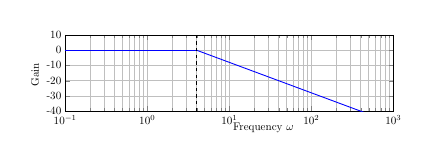
\begin{tikzpicture}
        [
            scale = 0.4,
            >=latex
        ]
        \begin{axis}
            [
                width=12cm,
                height=4cm,
                xmode=log,
                xmin=0.1, xmax=1000, ymin=-40, ymax=10,
                x label style={anchor=west},
                xlabel=Frequency $\omega$,
                y label style={anchor=south},
                ylabel=Gain $\deci \bel$,
                ytick={-40, -30, -20, -10, 0, 10},
                yticklabels={-40, -30, -20, -10, 0, 10},
                xmajorgrids=true,
                xminorgrids=true,
                ymajorgrids=true
            ]

            \addplot[thick, color=blue, domain=0.1:4]{0};  
            \addplot[thick, color=blue, domain=4:1000]{-20*log10(x)+12};   
            
            \addplot[dashed, color=black, domain=4:4]coordinates {(4, -40) (4, 10)};  
        \end{axis}
        
    \end{tikzpicture}


    % Phase
    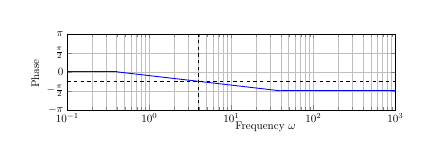
\begin{tikzpicture}
        [
            scale = 0.4,
            >=latex
        ]
        \begin{axis}
            [
                width=12cm,
                height=4cm,
                xmode=log,
                xmin=0.1, xmax=1000, ymin=-3.141, ymax=3.141,
                x label style={anchor=west},
                xlabel=Frequency $\omega$,
                y label style={anchor=south},
                ylabel=Phase $\rad$,
                ytick={-3.14, -1.57, 0, 1.57, 3.14},
                yticklabels={$-\pi$, $-\frac{\pi}{2}$, $0$, $\frac{\pi}{2}$, $\pi$},
                xmajorgrids=true,
                xminorgrids=true,
                ymajorgrids=true
            ]
            
            \addplot[thick, color=blue, domain=0.1:0.4]{0};  
            \addplot[thick, color=blue] coordinates{(0.4, 0) (40, -1.57)};   
            \addplot[thick, color=blue, domain=40:1000]{-1.57};  
            
            \addplot[dashed, color=black, domain=4:4] coordinates {(4, -3.14) (4, 3.14)};  
            \addplot[dashed, color=black, domain=0.1:1000]{-0.79};  

        \end{axis}
            
    \end{tikzpicture}
\end{center}



\end{minipage}
\hfill
\begin{minipage}[t]{0.48\columnwidth}
    \raggedright
    \subsubsection{Reelle Nullstelle} %TODO

    \begin{outline}
        \1 $H(s) = \frac{s + \alpha}{\alpha} = \frac{s}{\alpha} + 1 \cbl{= \frac{s + 5}{5}}$
            \2 Betrag $=$ Konstante mit Wert $0 \, \deci \bel$ von $\omega = 0$ bis $\omega = \alpha$; 
                für $\omega > \alpha$ Gerade mit Steigung $+ 20 \, \deci \bel / \Dek$ 
                durch Punkt mit Amplitude $0 \, \deci \bel$ und $\omega = \alpha$
            \2 Phase $=$ Konstante mit Wert $0$ bis $\omega < \frac{\alpha}{10}$; 
                für $\omega > 10 \alpha$ Konstante mit Wert $+ \frac{\pi}{2}$; dazwischen eine Gerade
                (bei $\omega = \alpha$ beträgt Phase $+ \frac{\pi}{4}$)
    \end{outline}


    \begin{center}
    % Gain
    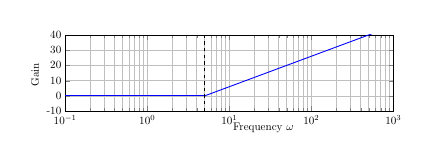
\begin{tikzpicture}
        [
            scale = 0.4,
            >=latex
        ]
        \begin{axis}
            [
                width=12cm,
                height=4cm,
                xmode=log,
                xmin=0.1, xmax=1000, ymin=-10, ymax=40,
                x label style={anchor=west},
                xlabel=Frequency $\omega$,
                y label style={anchor=south},
                ylabel=Gain $\deci \bel$,
                ytick={-10, 0, 10, 20, 30, 40},
                yticklabels={-10, 0, 10, 20, 30, 40},
                xmajorgrids=true,
                xminorgrids=true,
                ymajorgrids=true
            ]

            \addplot[thick, color=blue, domain=0.1:5]{0};  
            \addplot[thick, color=blue, domain=5:1000]{20*log10(x)-14};   
            
            \addplot[dashed, color=black, domain=5:5]coordinates {(5, -10) (5, 40)};  

        \end{axis}
        
    \end{tikzpicture}


    % Phase
    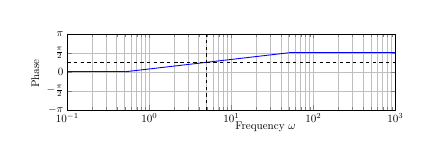
\begin{tikzpicture}
        [
            scale = 0.4,
            >=latex
        ]
        \begin{axis}
            [
                width=12cm,
                height=4cm,
                xmode=log,
                xmin=0.1, xmax=1000, ymin=-3.141, ymax=3.141,
                x label style={anchor=west},
                xlabel=Frequency $\omega$,
                y label style={anchor=south},
                ylabel=Phase $\rad$,
                ytick={-3.14, -1.57, 0, 1.57, 3.14},
                yticklabels={$-\pi$, $-\frac{\pi}{2}$, $0$, $\frac{\pi}{2}$, $\pi$},
                xmajorgrids=true,
                xminorgrids=true,
                ymajorgrids=true
            ]
            
            \addplot[thick, color=blue, domain=0.1:0.5]{0};  
            \addplot[thick, color=blue] coordinates{(0.5, 0) (50, 1.57)};   
            \addplot[thick, color=blue, domain=50:1000]{1.57};  
            
            \addplot[dashed, color=black, domain=5:5] coordinates {(5, -3.14) (5, 3.14)};  
            \addplot[dashed, color=black, domain=0.1:1000]{0.79};                 
        \end{axis}
            
    \end{tikzpicture}
\end{center}

\end{minipage}


\begin{minipage}[t]{0.48\columnwidth}
    \raggedright
    \subsubsection{Konj.-komplexe Pole} % TODO

    \begin{center}
    % Gain
    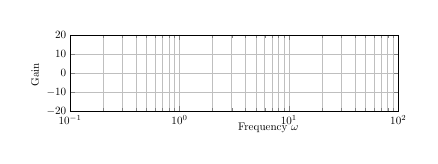
\begin{tikzpicture}
        [
            scale = 0.4,
            >=latex
        ]
        \begin{axis}
            [
                width=12cm,
                height=4cm,
                xmode=log,
                xmin=0.1, xmax=100, ymin=-20, ymax=20,
                x label style={anchor=west},
                xlabel=Frequency $\omega$,
                y label style={anchor=south},
                ylabel=Gain $\deci \bel$,
                xmajorgrids=true,
                xminorgrids=true,
                ymajorgrids=true
            ]

            \addplot[thick, color=blue, domain=0.1:100]{40};
        \end{axis}
        
    \end{tikzpicture}


    % Phase
    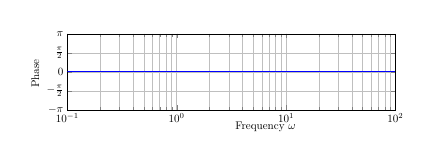
\begin{tikzpicture}
        [
            scale = 0.4,
            >=latex
        ]
        \begin{axis}
            [
                width=12cm,
                height=4cm,
                xmode=log,
                xmin=0.1, xmax=100, ymin=-3.141, ymax=3.141,
                x label style={anchor=west},
                xlabel=Frequency $\omega$,
                y label style={anchor=south},
                ylabel=Phase $\rad$,
                ytick={-3.14, -1.57, 0, 1.57, 3.14},
                yticklabels={$-\pi$, $-\frac{\pi}{2}$, $0$, $\frac{\pi}{2}$, $\pi$},
                xmajorgrids=true,
                xminorgrids=true,
                ymajorgrids=true
            ]
            
            \addplot[thick, color=blue, domain=0.1:100]{0};                 
        \end{axis}
            
    \end{tikzpicture}
\end{center}

\end{minipage}
\hfill
\begin{minipage}[t]{0.48\columnwidth}
    \raggedright
    \subsubsection{Konj.-komplexe Nullstellen} %TODO

    \begin{center}
    % Gain
    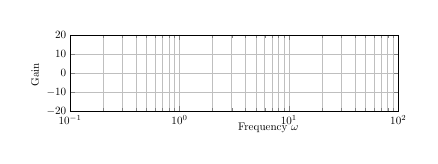
\begin{tikzpicture}
        [
            scale = 0.4,
            >=latex
        ]
        \begin{axis}
            [
                width=12cm,
                height=4cm,
                xmode=log,
                xmin=0.1, xmax=100, ymin=-20, ymax=20,
                x label style={anchor=west},
                xlabel=Frequency $\omega$,
                y label style={anchor=south},
                ylabel=Gain $\deci \bel$,
                xmajorgrids=true,
                xminorgrids=true,
                ymajorgrids=true
            ]

            \addplot[thick, color=blue, domain=0.1:100]{40};
        \end{axis}
        
    \end{tikzpicture}


    % Phase
    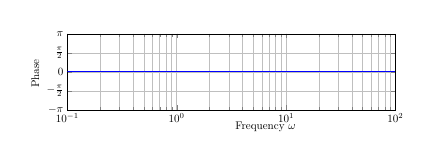
\begin{tikzpicture}
        [
            scale = 0.4,
            >=latex
        ]
        \begin{axis}
            [
                width=12cm,
                height=4cm,
                xmode=log,
                xmin=0.1, xmax=100, ymin=-3.141, ymax=3.141,
                x label style={anchor=west},
                xlabel=Frequency $\omega$,
                y label style={anchor=south},
                ylabel=Phase $\rad$,
                ytick={-3.14, -1.57, 0, 1.57, 3.14},
                yticklabels={$-\pi$, $-\frac{\pi}{2}$, $0$, $\frac{\pi}{2}$, $\pi$},
                xmajorgrids=true,
                xminorgrids=true,
                ymajorgrids=true
            ]
            
            \addplot[thick, color=blue, domain=0.1:100]{0};                 
        \end{axis}
            
    \end{tikzpicture}
\end{center}

\end{minipage}



\begin{minipage}[t]{0.48\columnwidth}
    \raggedright
    \subsubsection{Konstanter Faktor}

    \begin{outline}
        \1 $H(s) = \alpha \cdot e^{\jimg \beta} \cbl{= 3 \cdot e^{\jimg \frac{\pi}{2}}}$
            \2 Betrag $= 20 \cdot \log_{10}(\alpha) = \const$
            \2 Phase $= \beta = \const$
    \end{outline}
    
    \begin{center}
    % Gain
    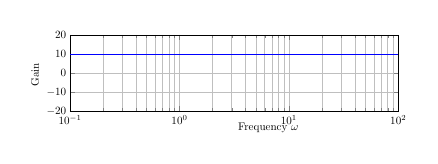
\begin{tikzpicture}
        [
            scale = 0.4,
            >=latex
        ]
        \begin{axis}
            [
                width=12cm,
                height=4cm,
                xmode=log,
                xmin=0.1, xmax=100, ymin=-20, ymax=20,
                x label style={anchor=west},
                xlabel=Frequency $\omega$,
                y label style={anchor=south},
                ylabel=Gain $\deci \bel$,
                xmajorgrids=true,
                xminorgrids=true,
                ymajorgrids=true
            ]

            % K_0
            \addplot[thick, color=blue, domain=0.1:100]{20*log10(3)};
        \end{axis}
        
    \end{tikzpicture}


    % Phase
    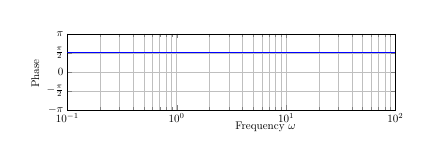
\begin{tikzpicture}
        [
            scale = 0.4,
            >=latex
        ]
        \begin{axis}
            [
                width=12cm,
                height=4cm,
                xmode=log,
                xmin=0.1, xmax=100, ymin=-3.141, ymax=3.141,
                x label style={anchor=west},
                xlabel=Frequency $\omega$,
                y label style={anchor=south},
                ylabel=Phase $\rad$,
                ytick={-3.14, -1.57, 0, 1.57, 3.14},
                yticklabels={$-\pi$, $-\frac{\pi}{2}$, $0$, $\frac{\pi}{2}$, $\pi$},
                xmajorgrids=true,
                xminorgrids=true,
                ymajorgrids=true
            ]
            
            % K_0
            \addplot[thick, color=blue, domain=0.1:100]{1.57};     

        \end{axis}
            
    \end{tikzpicture}
\end{center}
\end{minipage}
\hfill
\begin{minipage}[t]{0.48\columnwidth}
    \raggedright
    \subsubsection{Weitere Bemerkungen}


\end{minipage}


% \subsection{Vorgehen: Bodediagramm zeichnen}

% % Von Reglelungstechnik 2 (mit Anpassungen)
% Das Diagramm wird approximativ mit \textbf{Geraden} gezeichnet!

% \begin{outline}
%     \1 Übertragungsfunktion $H(s)$ in folgende Form bringen:
%         $$ G(s) = K \cdot (s)^v \cdot \frac{(1 + T_{n0} \cdot s)\cdot (1 + T_{n1} \cdot s) \cdot \ldots}
%         {(1 + T_{p0} \cdot s)\cdot (1 + T_{p1} \cdot s) \cdot \ldots} \cdot e^{- s T_t} $$
%         \2 Für $\omega = 0$ sind alle $(1 + T \cdot s) = 1 = 0 \, \deci \bel$
%         \2 Für $\omega = \frac{1}{T}$ sind alle  $(1 + T \cdot s) = 1 + \jimg = \sqrt{2} \cdot e^{\jimg \frac{\pi}{4}} 
%             = 3 \, \deci \bel \angle 45 \, \degree$ % CHECK or change
%     \1 Frequenzen der Nullstellen berechnen: $\omega = \frac{1}{T_n}$
%     \1 Frequenzen der Polstellen berechnen: $\omega = \frac{1}{T_p}$

%     \1 Jede \textbf{Nullstelle} bewirkt
%         \2 einen Knick um $+ 20 \, \deci \bel$ / Dekade \textbf{nach oben} im Amplitudengang
%         \2 einen Phasenhub von $+ 90 \, \degree$ über 2 Dekaden \textrightarrow\ $+ 45 \, \degree$ beim Knick
%     \1 Jede \textbf{Polstelle} bewirkt
%         \2 einen Knick um $- 20 \, \deci \bel$ / Dekade \textbf{nach unten} im Amplitudengang
%         \2 einen Phasenverlust von $- 90 \, \degree$ über 2 Dekaden \textrightarrow\ $- 45 \, \degree$ beim Knick
%     \1 Einzelne Faktoren einzeichnen \textrightarrow\ Wenn Faktor quadriert ist, zwei mal einzeichnen!
%     \1 Grafische Addition der Faktoren für gesamten Frequenzgang
% \end{outline}



\subsection{Bodediagramme mit Matlab}

\lstinputlisting{snippets/bode.m}
